\documentclass{article}
\usepackage[utf8]{inputenc}
\usepackage{amsmath}	% Advanced maths commands
\usepackage{amssymb}
\usepackage{natbib}
\usepackage{graphicx}
\bibliographystyle{abbrvnat}
\setcitestyle{authoryear,open={(},close={)}}

\renewcommand{\citealt}{\citep}

\title{Accelerated Implementations of the RIME for DDE Calibration and Bayesian Inference}
\author{Joshua van Staden}

\begin{document}

\maketitle
\section{Interferometry Basics}

The resolution of a single dish radio telescope is directly proportional to the diameter of its dish. Dishes can, however, become too large to be supported structurally. Some telescopes are able to overcome this, such as the Arecibo telescope, which consists of a giant dish built into the nearby landscape. However, even designs such as this displays limitations, such as not being able to rotate the dish to focus on a target. This issue can be resolved through telescope synthesis, whereby multiple telescopes have their outputs combined to emulate a larger telescope. This forms an interferometer.

Radio dishes in an interferometer are paired off into baselines. Both of the dishes in a baseline have their outputs correlated with each other, to generate a visibility. This has the effect of achieving a higher resolution than what either of the two telescopes can achieve individually. The resolution achieved by an interferometer is given by
\begin{equation}
\label{eq:resolution}
    \theta \approx 1.22 \frac{\lambda}{B} ,
\end{equation}
where $\theta$ is the resolution achieved, $\lambda$ is the wavelength observed, and $B$ is the longest baseline in the interferometer. Following Equation (\ref{eq:resolution}), one can see that, by making $B$ as large as possible, one can minimise $\theta$, which therefore shrinks pixel size and resolves smaller objects. This is the same effect as having a single dish telescope with a diameter of $B$, but it does not contain the drawback of having structural issues.

\begin{figure}
    \centering
    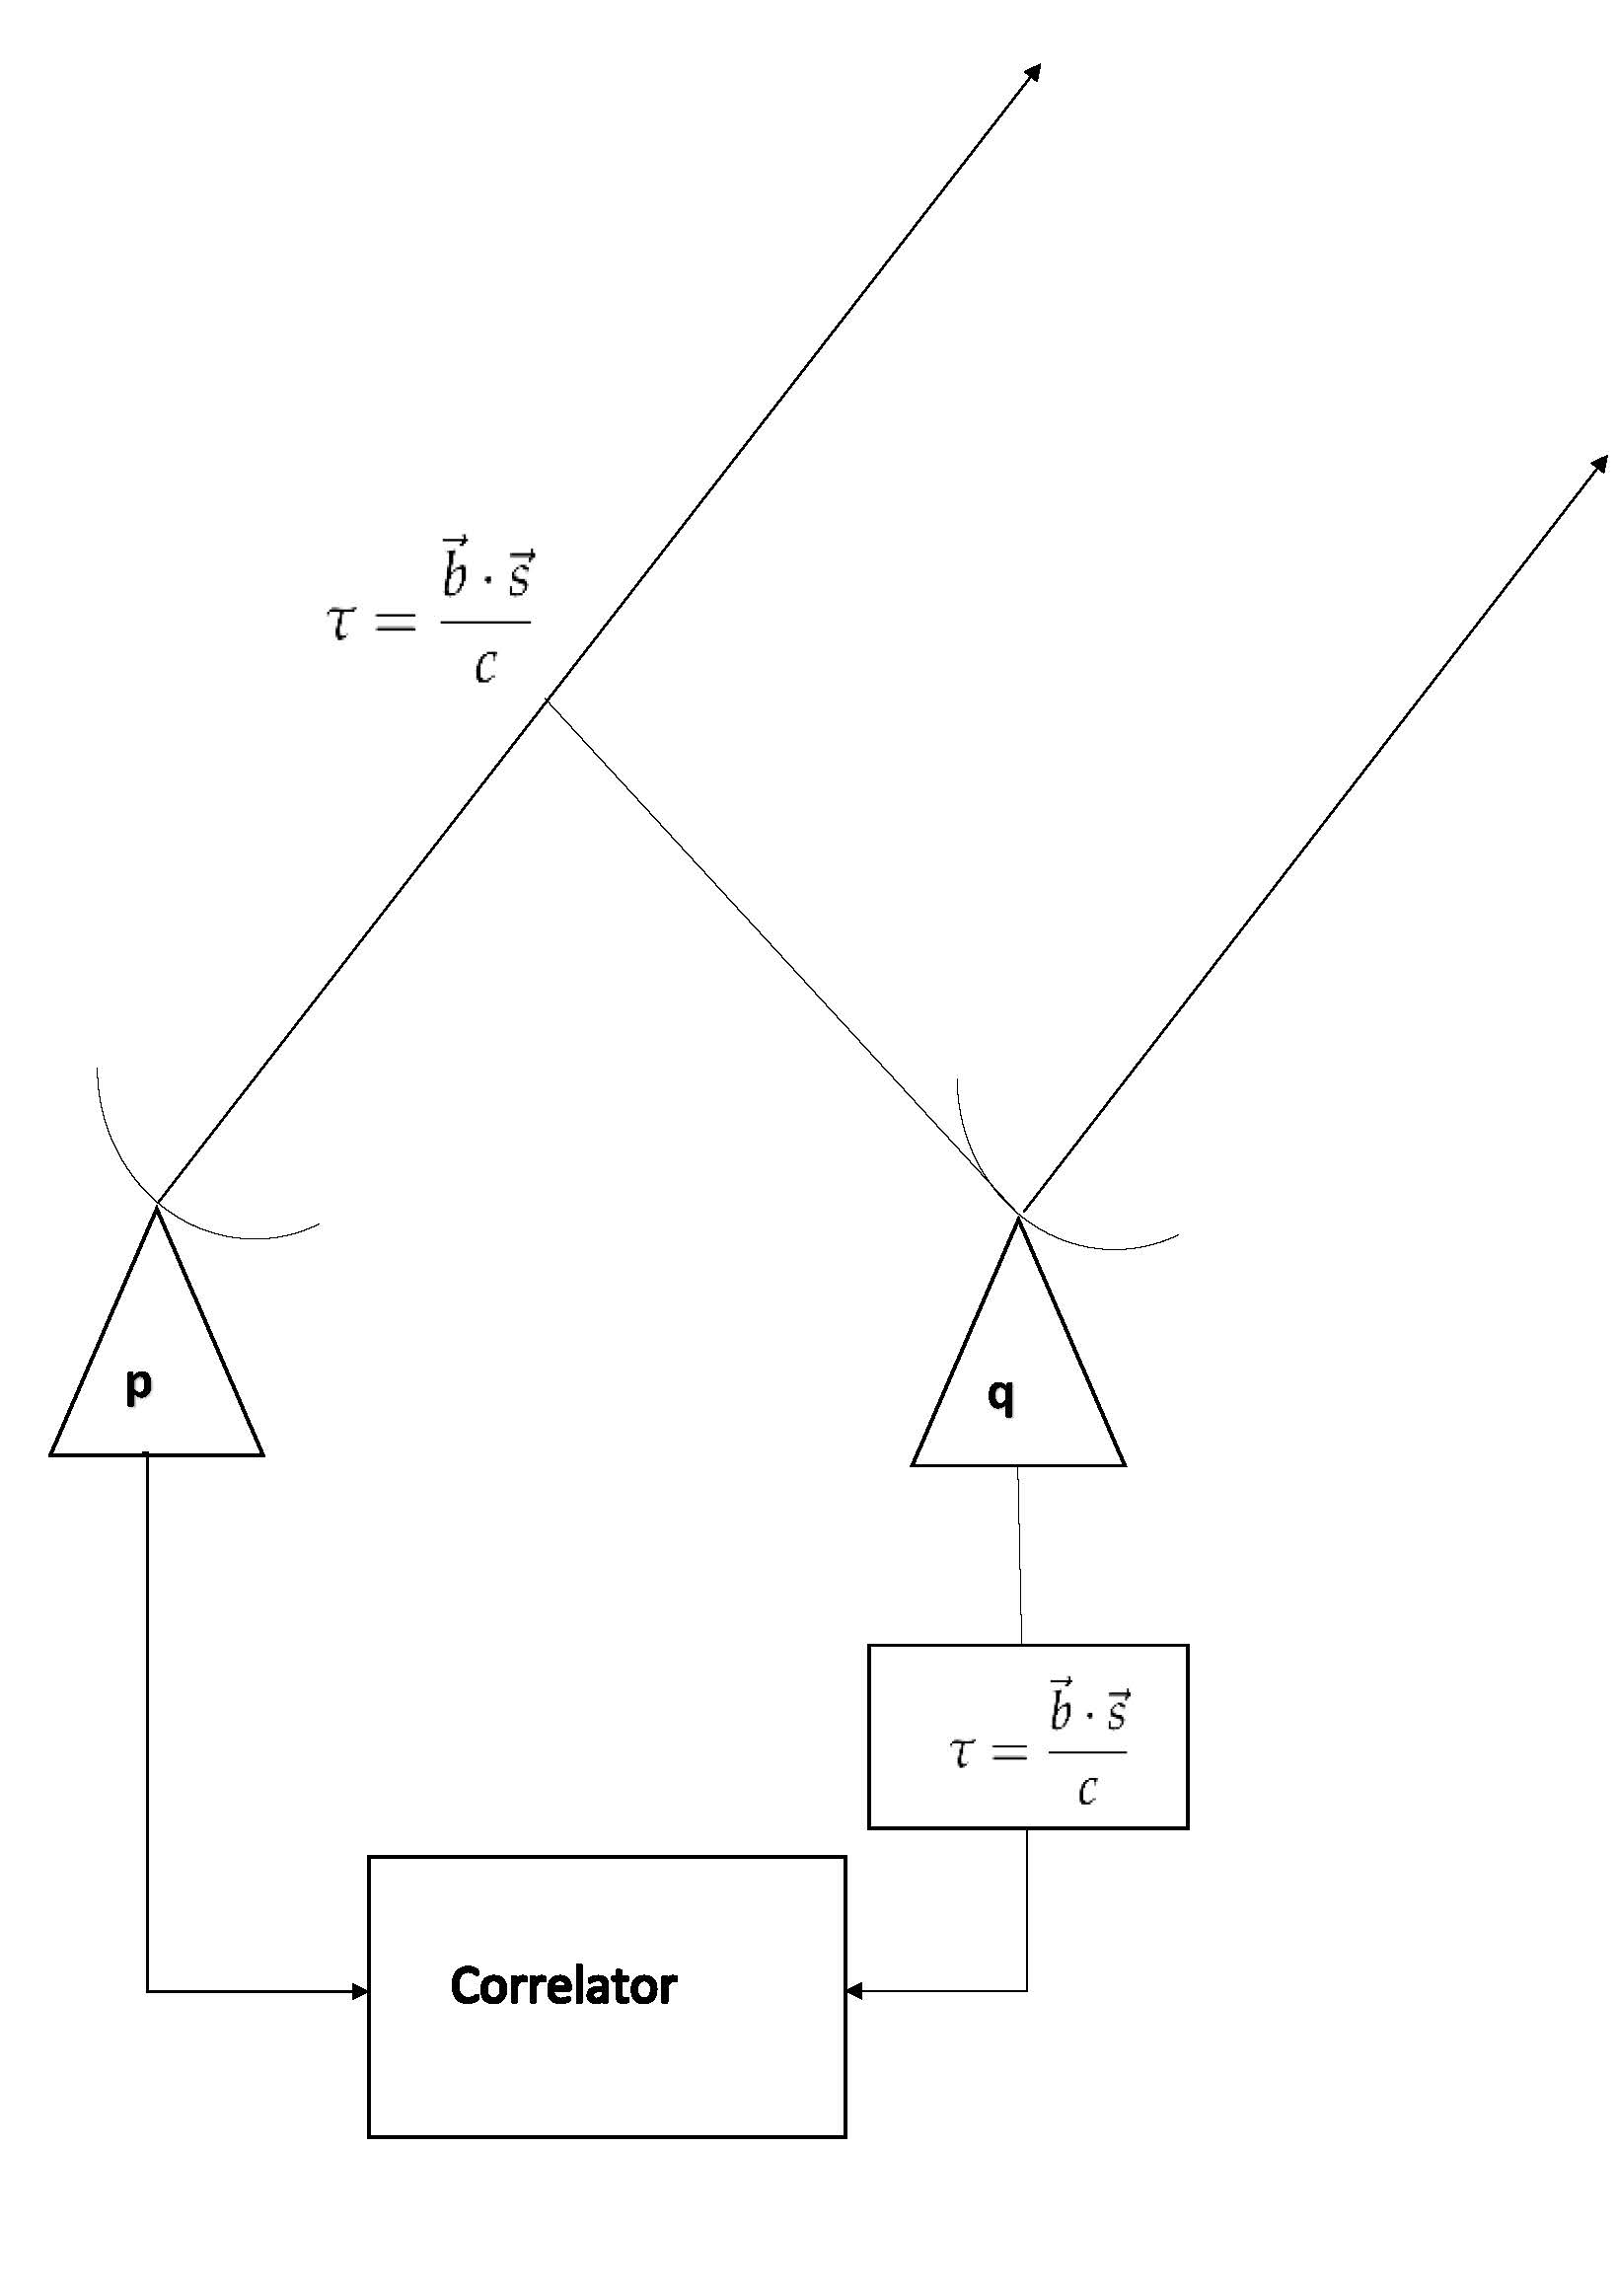
\includegraphics[width=0.4\textwidth]{DiagramTelescope.jpg}
    \caption{A diagram depicting the process of observing a source in the sky. Antenna $p$ and $q$ both observe the same source in the sky. A phase delay between the two observations $\tau = \frac{\Vec{b} \cdot \Vec{s}}{c}$ is introduced before the two signals get correlated at the correlator.}
    \label{fig:twoelement}
\end{figure}


 Figure \ref{fig:twoelement} illustrates a simple two-element interferometer. Both dishes are reading the same signal. The signal is detected at antennae $p$ and $q$. The outputs of these antennae are transmitted to a correlator, where a visibility is produced. Due to the fact that the telescopes are at two different points on the ground, the signal will arrive at each telescope at different times. This is known as the geometric delay (or phase delay), and is given as $\tau = \frac{\Vec{b} \cdot \Vec{s}}{c}$. To nullify the effect of the phase delay, the signal to the correlator gets delayed by the same geometric delay, as shown in the diagram.

The coordinates of the telescopes on the ground are measured using $(u, v, w)$ coordinates. These coordinates describe the telescopes' positions relative to one another, and are measured in wavelengths. The $w$ coordinate is the coordinate that lies orthogonal to the ground, and is $0$ if the telescopes are co-planar. The image space coordinates, which are denoted as $(l, m, n)$ coordinates, are the direction cosines of the $(u, v, w)$ coordinates, and is a unit vector denoting the coordinates in the image, with the $n$ coordinate lying in the direction of propagation of the signal. 

The visibilities measured by the telescopes, $\mathbf{V}(u, v, w)$, are related to the sky brightness distribution, $\mathbf{I}(l, m)$, by the following equation \citep{thompson2008}
\begin{equation}
\label{eq:vancittertzerniketheorem}
    \mathbf{V}(u, v, w) = \int \int _{-\infty}^\infty \mathbf{A}(l, m) \mathbf{I}(l, m) e^{-2 \pi \imath (ul + vm + w(n - 1))} \frac{dldm}{n} ,
\end{equation}
where $n = \sqrt{1 - l^2 - m^2}$, and $\mathbf{A}(l, m)$ is the point spread function, which arises due to limited sampling of the $uv$ plane. There are two aspects that are preventing the visibility being an exact 2D Fourier transform of the sky: namely the sampling function and the $w$ and $n$ coordinates. The $w$ and $n$ coordinates can be nullified if either:
\begin{itemize}
    \item The telescopes were coplanar, making $w$ zero, or
    \item we are imaging a very small region in the sky, making $n \approx 1$. 
\end{itemize}
Assuming $\mathbf{A}(l, m)$ were theoretically always $1$, and one of the above criteria were satisfied, Equation (\ref{eq:vancittertzerniketheorem}) could be approximated as a 2D Fourier transform. Due to the fact that $\mathbf{A}(l, m)$ is not $1$, this merely makes Equation (\ref{eq:vancittertzerniketheorem}) a 2D convolution. Deconvolution algorithms such as CLEAN\citep{hogbom1974aperture} exist which are able to undo this effect. 


By CLEANing the observed visibility, one can obtain the pure voltages read by the telescope. Unfortunately, these voltages contain many different effects that corrupt the source under study. The next section will discuss how calibration is done to correct for these effects and improve telescope sensitivity.

\section{Calibration}

\subsection{Calibration Techniques}

\subsubsection{First Generation Calibration}
First Generation Calibration (or 1GC, for short) is the process of pointing the telescope at a calibration source in the sky of known flux and position, calculating the gains on that source, and applying those gains to the target source. This technique was the main form of calibration before 1980 \citep{meqtrees}. This form of calibration is useful in solving for:
\begin{itemize}
    \item Absolute flux density
    \item Gain variations in the various frequency bands
    \item Phase delay
    \item Complex Antenna Gains
\end{itemize}
Calibration for these antenna effects will require that the calibrator source has certain properties. 

Firstly, the source should be bright. Due to the fact that as little time as possible should be spent on calibrating the telescope, as little time as possible is spent on observing the calibrator. A good SNR is required to detect the source itself, and a good SNR is achieved either through a long observation, or if the source under observation is brighter than the noise levels.

Secondly, it is preferable for the source to be unresolved. Resolved sources will have a brightness distribution varying with position, whereas an unresolved source will have a single brightness, which can be calibrated for.

Thirdly, the source must be close to the target field. Atmospheric effects can vary with position, so gains will therefore be different if the calibrator source is too far away.

Lastly, the source should  have a flat spectrum. For bandpass calibration, knowing the brightness in each frequency bin can allow one to solve for gains in each frequency.

\subsubsection{Second Generation Calibration}
At around 1980, \cite{2gc} proposed a new method of calibration, termed second-generation calibration (2GC), or self-calibration. This is a closed-loop method of calibration, which continuously updates a sky model of the observation. This has become widely used and led to dynamic ranges in the region of $10^4$ - $10^5$ \citep{meqtrees}. Self-calibration is mainly used in the process of computing direction-independent gains. 

Figure \ref{fig:selfcal} illustrates the process of self-calibration. This process iteratively evaluates the sky model obtained from 1GC and re-calibrates it until it fits the observed data to an acceptable level. The process of self-calibration begins by initialising a sky model from the data output from 1GC calibration. This sky model is Fourier transformed into model visibilities. These model visibilities are compared with the observed visibilities, and calibration is done to produce corrected visibilities. An inverse Fourier transform is done to produce a dirty image, which is deconvolved to produce a deconvolved image. This image will still have antenna gains affecting it, and so a source finder is used to try to isolate sources in the image. This source finder is used to update the sky model, and so the next iteration of selfcal would start, but with the sky model improving slightly at each iteration.

Selfcal is generally useful in computing direction independent complex antenna gains. Determining these antenna gains boils down to solving a non-linear least squares problem\citep{cubical}. Many algorithms exist, such as the Statistically Efficients and Fast Calibration (StEFCal) algorithm\citep{stefcal, mitchell2008stefcal} and the Levenberg-Marquardt \citep{levenberg1944method, marquardt1963algorithm} algorithm.

\subsubsection{Third Generation Calibration}
While 2GC is effective in solving for direction-independent complex antenna gains, the direction-dependent case is not solvable using this method. 3GC methods are still under research and have the potential to reach high dynamic ranges. These methods typically fall into one of two categories: physics-based approaches and heuristic-based approaches.

Physics-based DDE calibration is calibration done when the underlying physical phenomenon can be modelled and parameterised. One example is that of the primary antenna beam. \cite{mitra2015} modelled the primary beam of the Jansky Very Large Array (JVLA) at L-Band and, using Multi-Term Multi-Frequency Synthesis \citep{rau2011multi} and differential gains \citep{smirnov2011ddewsrt}, achieved an unprecendented dynamic range of 5 000 000 : 1. Another primary beam model has been created by \cite{khaneidos} of the MeerKAT primary antenna beam at L-Band. The analytic form of this was created using Zernike polynomials.

Heuristic-based DDE calibration is performed on DDEs where the underlying physical effect is not known, and is a form of solving for generic remaining DDEs. One such method of DDE calibration is \textit{peeling}\citep{noordam2004peeling}. 

\subsection{Measurement Equation}
The Radio Interferometer Measurement Equation (also known as the RIME), was originally formulated by \cite{hamaker1996} and later revisited by \cite{smirnov2011}. It is an intuitive equation that models the source and corruptions on the source using Jones calculus. Additionally, it provides a mathematical basis on which to model direction-independent effects acting on the source on the antenna side, as well as the direction-dependent effects happening nearer to the source. This paper will use the RIME as a calibration formalism for which to base the implementation on. This section aims to provide a summary of the derivation of the RIME, as well as an overview of how it handles the problem of DDEs.

\subsubsection{The Basic Discrete RIME}
The RIME begins by considering a quasi-monochromatic source. The flux density of this source $\vec{e} =\begin{pmatrix} e_x \\ e_y \end{pmatrix}$ with polarisation along the $x$ and $y$ axes can be modelled as a $2 \times 1$ vector, assuming the $z$ axis lies in the direction of propagation and can therefore be ignored.

Effects acting upon the source in the RIME are always assumed linear in nature. This allows us to model these effects as $2 \times 2$ Jones matrices ($\mathbf{J}$). The transformation undergone by a signal can therefore be represented as $\Vec{e'} = \mathbf{J}\Vec{e}$. Typically, the signal emanating from a source will undergo a number of these transformations during the course of its propagation from the source to its detection on Earth. The signal measured by the telescope is therefore a product of the different propagation matrices which distort the source signal. This is referred to as a Jones chain
\begin{equation}
\Vec{e'} = \mathbf{J}_{n} \mathbf{J}_{n-1}...\mathbf{J}_{2}\mathbf{J}_1 \Vec{e} .
\end{equation}
It is important to note that the first effect that the signal undergoes, $\mathbf{J}_1$, is the Jones matrix that is closest to the source $\Vec{e}$. The next Jones matrix, $\mathbf{J}_2$, acts upon the output of $\mathbf{J}_1\Vec{e}$. Therefore, $\mathbf{J}_n$ is the last effect to act on the signal, and so it is reasonable to assume that it acts on the signal at the antenna.

The visibility observed by a baseline consisting of antennae $p$ and $q$ consist of 4 voltages which are correlated as such:
\[
\langle v_{px} v^*_{qx} \rangle , \langle v_{px} v^*_{qy} \rangle , \langle v_{py} v^*_{qx} \rangle , \langle v_{py} v^*_{qy} \rangle ,
\]
where the angular brackets denote the averaging over time and frequency bins that occur when data sampling is performed. $v^*_{qx}$ denotes the complex conjugate of $v_{qx}$, the voltage measured by antenna $q$ in dimension $x$. This can be arranged into a visibility matrix $\mathbf{V}_{pq}$
\begin{equation}
\mathbf{V}_{pq} = 2\begin{pmatrix} 
\langle v_{px} v^*_{qx} \rangle && \langle v_{px} v^*_{qy} \rangle \\
\langle v_{py} v^*_{qx} \rangle && \langle v_{py} v^*_{qy} \rangle
\end{pmatrix} .
\end{equation}
For an explanation of the factor of $2$ at the beginning of the equation, see \cite{smirnov2011}. This can also be written as a matrix product of $\mathbf{V}_{p} = \begin{pmatrix} v_{px} \\ v_{py} \end{pmatrix}$ and $v^H_{q} = \begin{pmatrix} v^*_{qx} && v^*_{qy} \end{pmatrix}$, the conjugate (or Hermitian) transpose of $v_q$
\begin{equation}
\mathbf{V}_{pq} = 2 \langle \begin{pmatrix} v_{px} \\ v_{py} \end{pmatrix} \begin{pmatrix} v^*_{qx} && v^*_{qy} \end{pmatrix} \rangle .
\end{equation}
Considering that the source is being measured by two separate antennae, the same source $\Vec{e}$ will undergo two different travel paths to each antenna, represented as their own Jones matrices. This is shown as
\begin{align}
\mathbf{V}_{pq} &= 2\langle \mathbf{J}_p \Vec{e} ( \mathbf{J}_q \Vec{e} ) ^H  \rangle \\
&= 2\langle \mathbf{J}_p (\Vec{e} \Vec{e}^H) \mathbf{J}_q^H \rangle . \label{eq:difpaths}
\end{align}
The significance of the term $\Vec{e}\Vec{e}^H$ is that it has a close relation with the Stokes parameters\citep{bornwolf1964, thompson2008}. This is given as
\begin{align}
2\Vec{e}\Vec{e}^H &= 2\begin{pmatrix} 
\langle e_x e_x^* \rangle && \langle e_x e_y^* \rangle \\
\langle e_y e_x^* \rangle && \langle e_y e_y^* \rangle
\end{pmatrix}
\\
&= \begin{pmatrix}
I + Q && U + \imath V \\
U - \imath V && I - Q
\end{pmatrix} \\
&= \mathbf{B} .
\end{align}
$\mathbf{B}$, the brightness matrix, simply represents the source flux density in each polarisation. Rewriting Equation (\ref{eq:difpaths}) in terms of the brightness matrix, we get
\begin{equation}
\mathbf{V}_{pq} = \mathbf{J}_p \mathbf{B} \mathbf{J}_q^H .
\end{equation}
This is the basic form of the RIME, describing a single source undergoing a single linear transformation. One can use Jones chains to recursively define multiple linear transformations, giving way to what is referred to as the ``onion'' form of the RIME\citep{smirnov2011}
\begin{equation}
\mathbf{V}_{pq} = \mathbf{J}_{pn}(\mathbf{J}_{pn-1}(...(\mathbf{J}_{p2}(\mathbf{J}_{p1} \mathbf{B} \mathbf{J}^H_{q1})\mathbf{J}^H_{q2})...)\mathbf{J}^H_{qn-1})\mathbf{J}^H_{qn} .
\end{equation} 

As mentioned above, the Jones matrices that occur closer to the source are positioned closer to the brightness matrix in the Jones chain, and those that occur closer to the telescope are positioned at the ends of the equation. This form of the RIME describes a single source being corrupted by multiple effects. 

The RIME for multiple sources is simply a summation across each source
\begin{equation}
\label{eq:multiplesources}
    \mathbf{V}_{pq} = \sum_s \mathbf{J}_{sp} \mathbf{B}_s \mathbf{J}^H_{sq} ,
\end{equation}
where $\mathbf{J}_{sp}$ denotes the Jones terms for antenna $q$ at source $s$. 

With this in mind, it is possible to separate the Jones matrices into two different components, namely $\mathbf{G}_p$, the source-independent ``antenna'' Jones matrices, and $\mathbf{E}_p$, the source-dependent ``source'' Jones matrices. This allows us to rewrite Equation (\ref{eq:multiplesources}) as
\begin{equation}
\label{eq:discreteRIME}
\mathbf{V}_{pq} = \mathbf{G}_p (\sum_s \mathbf{E}_{sp} \mathbf{B} \mathbf{E}_{sq}^H)\mathbf{G}^H_{q} .
\end{equation}
$\mathbf{G}_p$ does not need to be included in the summation, as it remains constant across all sources. Among the Jones matrices in $\mathbf{E}_{sp}$, there exists a matrix $\mathbf{K}_{sp}$, which represents the phase delay, which is scalar. Due to this, it commutates with all other matrices. When the phase delay is multiplied with the source brightness $\mathbf{B}$, one gets the source coherency $\mathbf{X}_{spq}$. Substituting the source coherency into the RIME (Equation (\ref{eq:discreteRIME})), one gets
\begin{equation}
\label{eq:sourcecoherency}
\mathbf{V}_{pq} = \mathbf{G}_p (\sum_s \mathbf{E}_{sp} \mathbf{X}_{spq} \mathbf{E}_{sq}^H)\mathbf{G}^H_{q} ,
\end{equation}
where $\mathbf{X}_{spq}$ denotes the source coherency at source $s$ and baseline corresponding to antennae $p$ and $q$.

\subsubsection{The Continuous RIME}
Equation (\ref{eq:sourcecoherency}) gives the RIME in terms of the source coherency for a discrete number of sources in the sky. Considering the sky should rather be thought of as consisting of a continuous distribution of sources, this is not a practical form of the RIME for analytic purposes. Equation (\ref{eq:sourcecoherency}) can be extended to the continuous case by assuming $\mathbf{B}$ to be a continuous function of $\phi$, the unit direction vector. The same would be attached to the Jones terms. The continuous RIME for brightness matrix distribution $\mathbf{B}(\phi)$ with continuous Jones matrix distributions $\mathbf{J}(\phi)$ acting on it is given as an integration over the unit sphere
\begin{equation}
\mathbf{V}_{pq} = \int \int_{4\pi} \mathbf{J}_p(\phi) \mathbf{B}(\phi) \mathbf{J}^H_q(\phi) d\phi .
\end{equation}
This, however, is not very tractable. To get around this, one would perform a sine projection of the sphere onto the plane $(l,m)$, which is tangential to the field centre. Performing this sine projection, we end up with
\begin{equation}
\label{eq:continuousjones}
\mathbf{V}_{pq} = \int \int _{lm} \mathbf{J}_p(l, m) \mathbf{B}(l, m) \mathbf{J}^H_q(l, m) \frac{dldm}{n} ,
\end{equation}
where $n = \sqrt{1 - l^2 - m^2}$. We can then decompose $\mathbf{J}_p(l, m)$ into the respective DDEs, DIEs, and the phase delay term
\begin{align}
\mathbf{J}_p(l, m) &= \mathbf{G}_p \mathbf{E}_p(l, m) \mathbf{K}_p(l, m) \\
&= \mathbf{G}_p \mathbf{E}_p(l, m) e^{-2 \pi \imath (u_pl + v_pm + w_p(n-1))} .
\label{eq:continuoussplit}
\end{align}
Substituting Equation (\ref{eq:continuoussplit}) into Equation (\ref{eq:continuousjones}), we get
\begin{equation}
\mathbf{V}_{pq} = \mathbf{G}_p (\int \int_{lm} \frac{1}{n} \mathbf{E}_p(l, m) \mathbf{B}(l,m) \mathbf{E}^H_q(l, m) e^{-2 \pi \imath (u_{pq}l + v_{pq}m + w_{pq}(n-1))} dldm) \mathbf{G}^H_q .
\end{equation}
This is one form of a general, full-sky RIME. It is a type of three-dimensional Fourier transform, but the $\frac{1}{n}$ term and the $e^{-2 \pi \imath w_{pq}(n-1)}$ term stop it from being a regular, two-dimensional Fourier transform. In order to convert this into a two-dimensional Fourier transform, one can create a $\mathbf{W}_p$ term, where $\mathbf{W}_p = \frac{1}{\sqrt{n}} e^{-2 \pi \imath w_{p}(n-1)}$. This can be thought of as a Jones matrix in and of itself. With this in mind, one can create a new term $\Tilde{\mathbf{E}}_{p}(l,m) = \mathbf{E}_p(l, m) \mathbf{W}_p(l, m)$. This can then be placed into the RIME
\begin{equation}
\mathbf{V}_{pq} = \mathbf{G}_p (\int \int_{lm}\Tilde{\mathbf{E}}_p(l, m) \mathbf{B}(l,m) \Tilde{\mathbf{E}}^H_q(l, m) dldm) \mathbf{G}^H_q  .
\end{equation}
This can be shortened to
\begin{equation}
\label{eq:rimebpq}
\mathbf{V}_{pq} = \mathbf{G}_p (\int \int_{lm}\mathbf{B}_{pq}(l,m) dldm) \mathbf{G}^H_q ,
\end{equation}
where
\[
\mathbf{B}_{pq}(l, m) = \Tilde{\mathbf{E}}_p(l, m) \mathbf{B}(l,m) \Tilde{\mathbf{E}}^H_q(l, m)
\]
Equation (\ref{eq:rimebpq}) is a calibration for $\mathbf{B}_{pq}$. The significance of $pq$ being attached to $\mathbf{B}$ is that it makes the assumption that $\mathbf{B}$ varies per baseline. The cause for this variance between baselines is caused by the different DDE terms $\Tilde{\mathbf{E}}_p(l, m)$ and $\Tilde{\mathbf{E}}^H_q(l, m)$ that occur per baseline. This is a violation of the fundamental assumption of self calibration, which is that every antenna is measuring the Fourier transform of the same sky. Therefore, in order to maintain this assumption, another assumption must be made, which is that the DDE terms $\Tilde{\mathbf{E}}_p(l, m)$ must remain constant across all baselines. This assumption can be shown mathematically as
\[
\mathbf{B}_{pq}(l, m) \equiv \mathbf{B}_{app}(l, m) = \mathbf{E}(l, m)\mathbf{B}(l, m) \mathbf{E}^H(l, m) ,
\]
where $\mathbf{B}_{app}(l, m)$ represents the apparent brightness, \textit{i.e.} the brightness observed assuming all DDEs remain constant, and $\mathbf{E}(l, m)$ and $\mathbf{E}^H(l, m)$ are no longer antenna dependent. It is important to note that, while $\mathbf{E}(l, m)$ and $\mathbf{E}^H(l, m)$ are not antenna dependent, $\mathbf{G}_{p}$ and $\mathbf{G}^H_q$ will still remain antenna dependent. The reason for this is that the $\mathbf{E}$ terms occur at the source, and we are assuming that each telescope is observing the same source. Considering the $\mathbf{G}$ terms are occurring at the telescope, this assumption has no bearing on these terms.

With this assumption in mind, we can rewrite the full-sky RIME as 
\begin{equation}
\mathbf{V}_{pq} = \mathbf{G}_{p} \mathbf{X}_{pq} \mathbf{G}^H_q ,
\end{equation}
where $\mathbf{X}_{pq} = \mathbf{X}(u_{pq}, v_{pq})$ is the element-by-element two-dimensional Fourier transform of the brightness matrix function $\mathbf{B}_{app}(l, m)$.

The RIME provides a rigorous framework on which to model polarised sources observed by an antenna. It provides a way to model visibilities observed of a source undergoing direction-dependent gains, while still modelling the direction-independent antenna gains. 


\bibliography{example.bib}
\end{document}
